\documentclass[a4paper, 11pt]{article}
\usepackage{geometry}
\geometry{letterpaper, margin=1in}
\usepackage{amsmath}
\usepackage{amssymb}  
\usepackage{amsthm}
\usepackage{ulem} 
\usepackage{graphicx}
\usepackage{enumitem} % use for making lettered list 
\usepackage{bbm} % use for making the 1 identity operator EX: \mathbbm{1}
\usepackage{subfig} 
\graphicspath{ {images/} }

% format to allow bolded theorems, corollaries, etc... 
\newtheorem*{theorem}{Theorem}
\newtheorem*{corollary}{Corollary}
\newtheorem*{lemma}{Lemma}
\newtheorem*{definition}{Definition}
\newtheorem*{Example}{Example} 
\newtheorem*{Remark}{Remark}

% stop typing \mathbb a thousand times 
\newcommand{\R}{\mathbb{R}}
\newcommand{\C}{\mathbb{C}}
\newcommand{\F}{\mathbb{F}}
\newcommand{\Mat}[2]{\mathcal{M}_{#1\times#2}}

% change margins for solution
\newenvironment{solution}{%
	\begin{list}{}{%
			\setlength{\topsep}{0pt}%
			\setlength{\leftmargin}{1.5cm}%
			\setlength{\rightmargin}{1.5cm}%
			\setlength{\listparindent}{\parindent}%
			\setlength{\itemindent}{\parindent}%
			\setlength{\parsep}{\parskip}%
		}%
		\item[]}{\end{list}}

\begin{document}
%Header-Make sure you update this information!!!!
\noindent
\large\textbf{Dynein Model Explanation and Theory} \hfill \textbf{John Waczak} \\
\normalsize Dr. David Roundy \hfill  Date: \today \\
\par\noindent\rule{\textwidth}{0.4pt} \\


\section*{General Theory}
\noindent Our model for dyenin consists of a system of domains treated as spheres connected by massless rigid rods. Because dynein works inside of cells, it's aqueous environment exaggerates the forces due to drag and adds an extra random force due to collisions with water molecules. This results in the following equation of motion known as the Langevin equation:
\begin{equation}
  m\ddot{\mathbf{x}} = \mathbf{F}_\text{interact} -\gamma\dot{\mathbf{x}}+\mathbf{R} 
\end{equation}
In our simulation, we use Brownian dynamics which assumes that the drag great enough so that acceleration may be neglected and, therefore, equation (1) reduces to
\begin{equation}
  \dot{\mathbf{x}} = \frac{1}{\gamma}\left(\mathbf{F}_\text{interact}+\mathbf{R}\right) 
\end{equation}
where $\mathbf{x}$ is the position of the Brownian particle and $\mathbf{R}$ is the random force due to water molecule collisions. $\gamma$ is the drag coefficient and depends on the radius of the Brownian particle. $\mathbf{F}_\text{interact}$ is the force of interaction between the particles. For our purposes, this interaction is composed of two separate forces. Our massless rods are rigid and therefore there is a tension force between adjacent domains responsible for maintaining the length constraint. We also apply a Hooke's law restorative torque with a magnitude given by
\begin{equation}
  \Gamma_i = c_i(\varphi_i - \varphi_{i, \text{eq}})
\end{equation}
where $c_i$ is a constant and $\varphi_{i,\text{eq}}$ the equilibrium angle for the $i^\text{th}$ domain. The forces that these torques exert move the protein towards a preferred configuration and helps generate directed motility. Given this information, we can now discuss how these forces are determined for each of the simulation's possible states.
\pagebreak

\section*{One bound Model}
The following figure shows the model in the one bound configuration.\\
\begin{figure}[!hbt]
  \centering
  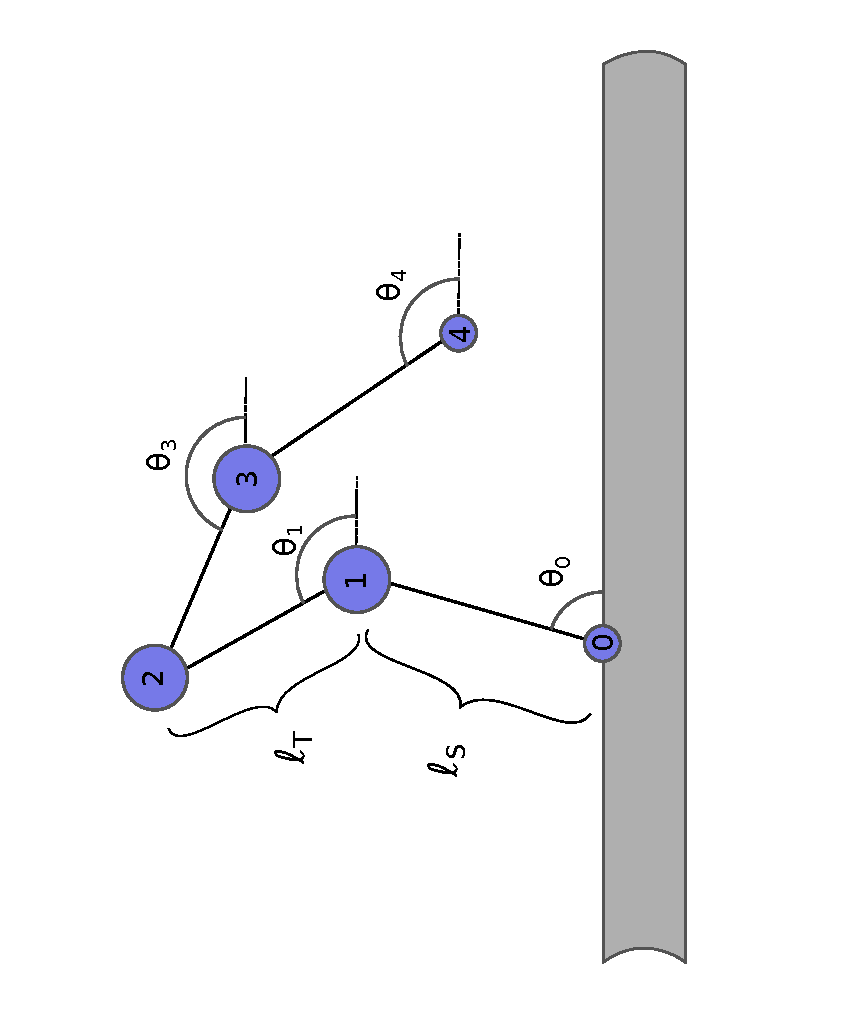
\includegraphics[width=0.6\columnwidth]{onebound}
  \caption{The dynein model in the one bound state } 
\end{figure}

\noindent Here $\ell_S, \ell_T$ are fixed stalk and tail lengths. We have chosen the angles $\{\theta_i\}$ as they are the most convenient and lead to a description of the position of each domain that requires only one angle and an adjacent position, that is
\begin{align}
  x's \quad &\begin{cases}
    x_0 = x_\text{bound} \\
    x_1 = x_0 + \ell_S \cos\theta_0 \\
    x_2 = x_1 + \ell_T \cos\theta_1 \\
    x_3 = x_2 + \ell_T \cos(\pi-\theta_3) = x_2 - \ell_T\cos\theta_3 \\
    x_4 = x_3 + \ell_S \cos(\pi-\theta_4) = x_3 - \ell_S\cos\theta_4
  \end{cases} \\
  y's \quad &\begin{cases}
    y_0 = 0 \\
    y_1 = y_0 + \ell_S\sin\theta_0 \\
    y_2 = y_1 + \ell_T\sin\theta_1 \\
    y_3 = y_2 - \ell_T\sin\theta_3 \\
    y_4 = y_3 - \ell_S\sin\theta_4 
  \end{cases}
\end{align} 

 \noindent Because equation (2) relates the forces on each domain to its velocity we need the time derivative of the above equations. 
 \begin{equation}
   \dot{x}'s \quad \begin{cases}
     \dot{x}_0 = 0 \\
     \dot{x}_1 = \dot{x}_0-\ell_S\sin\theta_0 \dot{\theta}_0 \\
     \dot{x}_2 = \dot{x}_1-\ell_T\sin\theta_1 \dot{\theta}_1 \\
     \dot{x}_3 = \dot{x}_2+\ell_T\sin\theta_3 \dot{\theta}_3 \\
     \dot{x}_4 = \dot{x}_3+\ell_S\sin\theta_4 \dot{\theta}_4
   \end{cases} \\
 \end{equation}
 \begin{equation}
   \dot{y}'s \quad \begin{cases}
     \dot{y}_0 = 0 \\
     \dot{y}_1 = \dot{y}_0 + \ell_S\cos\theta_0\dot{\theta}_0 \\
     \dot{y}_2 = \dot{y}_1 + \ell_T\cos\theta_1\dot{\theta}_1 \\
     \dot{y}_3 = \dot{y}_2 - \ell_T\cos\theta_3\dot{\theta}_3 \\
     \dot{y}_4 = \dot{y}_3 - \ell_S\cos\theta_4\dot{\theta}_4
   \end{cases} 
 \end{equation}



\end{document} 
